\documentclass{article}
\usepackage{tikz}

\begin{document}
   The stepper motor accelerates and decelerates following a trapezoidal speed profile. Since the stepper motor turns in discrete steps  a algorithm is utilized 
   which can generate the pulses neccesary to approximate the linear increase of the velocity.

   \section{theory}
   \begin{figure}
        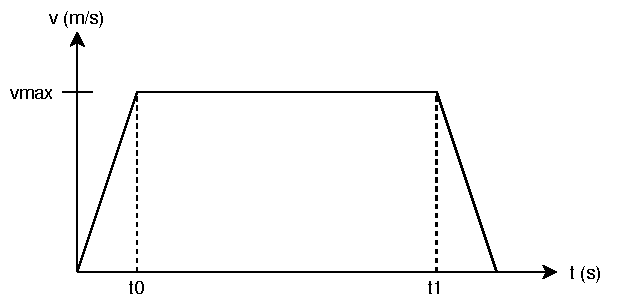
\includegraphics[width=\linewidth]{graph.pdf}
   \end{figure}
    
\end{document}